\documentclass[11pt,a4paper]{article}

\usepackage[utf8]{inputenc}
\usepackage[T1]{fontenc}
\usepackage{amsmath,amssymb}
\usepackage{geometry}
\usepackage{hyperref}
\usepackage{caption}
\usepackage{tikz}
\usepackage{algorithm}
\usepackage{algpseudocode}
\usetikzlibrary{shapes, arrows.meta, positioning, calc, decorations.pathreplacing, backgrounds}

\geometry{margin=1in}

\title{\textbf{Method 2: Dynamic Filling Function using Pivot and LDW}}
\author{Research Team}
\date{\today}

\begin{document}

\maketitle

\begin{abstract}
This document details Method 2, a highly robust dynamic filling function designed to map discrete evaluation scores ($s \in [0, 100]$) to structural search parameters ($ef$). Addressing the inherent sparsity of empirical tuning data, Method 2 employs a combination of Pivot-bound ocean extrapolation for boundary conditions and Inverse Distance Weighting (IDW/LDW) for internal interpolation (holes). This ensures localized spike preservation while maintaining global smoothness.
\end{abstract}

\section{Theoretical Formulation}

Let the domain of possible scores be defined as $\mathcal{S} = \{0, 1, \dots, 100\}$. During the parameter tuning phase, we observe optimal $ef$ values only at a sparse subset of scores. Let this set of known optimal pairs be $\mathcal{K} = \{(s_i, ef_i)\}_{i=1}^N$.

To define the boundaries, we establish the minimum and maximum observed scores:
\begin{align*}
    s_{min} &= \min_{(s_i, ef_i) \in \mathcal{K}} s_i \\
    s_{max} &= \max_{(s_i, ef_i) \in \mathcal{K}} s_i
\end{align*}

Method 2 systematically computes the imputed parameter value $\hat{ef}(s)$ for all $s \in \mathcal{S}$ through a piece-wise interpolation and extrapolation strategy.

\subsection{Pivot and LDW Equations}
The function strictly bounds extrapolation in the unobserved lower and upper extremes (the ``Oceans'') using predefined safe anchors, $\text{Pivot}_L$ and $\text{Pivot}_R$. For missing data within the observed range (the ``Holes''), it applies Local Distance Weighting (LDW), effectively distributing the influence of known spikes based on the inverse square distance.

For any score $s \in \mathcal{S}$, the filling function is explicitly defined as:
\begin{equation}
\hat{ef}(s) = 
\begin{cases} 
\max\left( ef_{s_{min}}, \, \text{Pivot}_L \right) & \text{if } s < s_{min} \quad \text{(Left Ocean)} \\[8pt]
\min\left( ef_{s_{max}}, \, \text{Pivot}_R \right) & \text{if } s > s_{max} \quad \text{(Right Ocean)} \\[8pt]
ef_s & \text{if } s \in \mathcal{K} \quad \text{(Spike Preservation)} \\[8pt]
\displaystyle \frac{\sum_{i \in \mathcal{K}} w_i(s) \cdot ef_i}{\sum_{i \in \mathcal{K}} w_i(s)} & \text{otherwise} \quad \text{(LDW for Holes)}
\end{cases}
\end{equation}

where the LDW weights $w_i(s)$ are computed using the inverse-square distance:
\begin{equation}
w_i(s) = \frac{1}{|s - s_i|^2}
\end{equation}

This inverse-square relation ensures that proximal known points heavily dictate the parameter value, while distant points yield a smooth asymptotic influence.

\section{Algorithmic Visualization}

The following diagram illustrates the distinct operational regimes of Method 2 across the 1D score space $\mathcal{S} \in [0, 100]$. Notice how the Left Ocean applies a $\max$ function (stepping up to $\text{Pivot}_L$), while the Right Ocean applies a $\min$ function (stepping down to $\text{Pivot}_R$).

\begin{figure}[htbp]
    \centering
    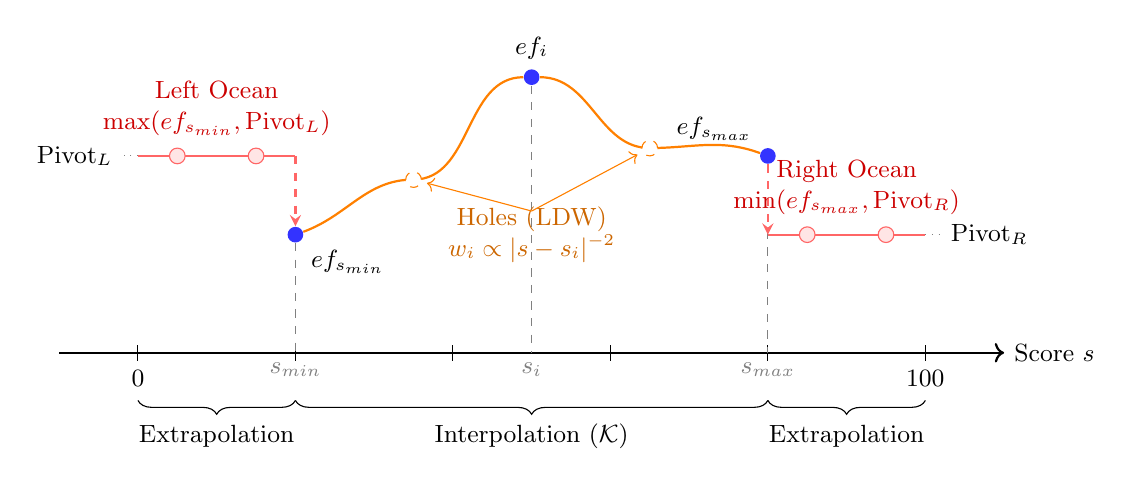
\begin{tikzpicture}[
        scale=1.0,
        every node/.style={font=\small},
        known/.style={circle, fill=blue!80, inner sep=2pt},
        hole/.style={circle, draw=orange, fill=white, inner sep=2pt, dashed},
        ocean/.style={circle, draw=red!60, fill=red!10, inner sep=2pt}
    ]

    % Axis
    \draw[thick, ->] (-1, 0) -- (11, 0) node[right] {Score $s$};
    \foreach \x in {0, 2, ..., 10} {
        \draw (\x, -0.1) -- (\x, 0.1);
    }
    \node[below] at (0, -0.1) {0};
    \node[below] at (10, -0.1) {100};

    % Known Data Points (Spikes)
    \node[known, label=below right:{$ef_{s_{min}}$}] (k1) at (2, 1.5) {};
    \node[known, label=above:{$ef_i$}] (k2) at (5, 3.5) {};
    \node[known, label=above left:{$ef_{s_{max}}$}] (k3) at (8, 2.5) {};
    
    \draw[dashed, gray] (k1) -- (2,0) node[below] {$s_{min}$};
    \draw[dashed, gray] (k2) -- (5,0) node[below] {$s_i$};
    \draw[dashed, gray] (k3) -- (8,0) node[below] {$s_{max}$};

    % Left Ocean Extrapolation (MAX function -> steps UP to Pivot_L)
    % Assuming Pivot_L = 2.5 which is > ef_{s_min} (1.5)
    \draw[red!60, thick] (0, 2.5) -- (2, 2.5);
    \draw[red!60, thick, dashed, -stealth] (2, 2.5) -- (k1);
    \node[draw=none, text=red!80!black, align=center] at (1, 3.1) {Left Ocean\\$\max(ef_{s_{min}}, \text{Pivot}_L)$};
    \node[ocean] at (0.5, 2.5) {};
    \node[ocean] at (1.5, 2.5) {};
    \draw[gray, dotted] (0, 2.5) -- (-0.2, 2.5) node[left, text=black] {$\text{Pivot}_L$};

    % LDW Interpolation (Holes)
    \draw[orange, thick, smooth] (k1) to[out=20, in=180] (3.5, 2.2) to[out=0, in=180] (k2);
    \draw[orange, thick, smooth] (k2) to[out=0, in=180] (6.5, 2.6) to[out=0, in=160] (k3);
    
    \node[hole] (h1) at (3.5, 2.2) {};
    \node[hole] (h2) at (6.5, 2.6) {};
    
    \node[draw=none, text=orange!80!black, align=center] at (5, 1.5) {Holes (LDW)\\$w_i \propto |s - s_i|^{-2}$};
    \draw[->, orange, shorten >=2pt] (5, 1.8) -- (h1);
    \draw[->, orange, shorten >=2pt] (5, 1.8) -- (h2);

    % Right Ocean Extrapolation (MIN function -> steps DOWN to Pivot_R)
    % Assuming Pivot_R = 1.5 which is < ef_{s_max} (2.5)
    \draw[red!60, thick, dashed, -stealth] (k3) -- (8, 1.5);
    \draw[red!60, thick] (8, 1.5) -- (10, 1.5);
    \node[draw=none, text=red!80!black, align=center] at (9, 2.1) {Right Ocean\\$\min(ef_{s_{max}}, \text{Pivot}_R)$};
    \node[ocean] at (8.5, 1.5) {};
    \node[ocean] at (9.5, 1.5) {};
    \draw[gray, dotted] (10, 1.5) -- (10.2, 1.5) node[right, text=black] {$\text{Pivot}_R$};

    % Braces for domains
    \draw [decorate,decoration={brace,amplitude=5pt,mirror,raise=4ex}]
      (0,0) -- (2,0) node [midway,yshift=-3em] {Extrapolation};
      
    \draw [decorate,decoration={brace,amplitude=5pt,mirror,raise=4ex}]
      (2,0) -- (8,0) node [midway,yshift=-3em] {Interpolation ($\mathcal{K}$)};
      
    \draw [decorate,decoration={brace,amplitude=5pt,mirror,raise=4ex}]
      (8,0) -- (10,0) node [midway,yshift=-3em] {Extrapolation};

    \end{tikzpicture}
    \caption{Topology of Method 2 mapping $ef$ values to scores. The space is distinctly partitioned into two extrapolation regimes (Left/Right Oceans bounded by Pivots) and an internal interpolation regime (Holes resolved via LDW). Notice the Left Ocean steps UP to satisfy $\max(ef, \text{Pivot}_L)$ as a lower-bound safety net, while the Right Ocean steps DOWN to satisfy $\min(ef, \text{Pivot}_R)$ to cap the computational cost.}
    \label{fig:fill_viz}
\end{figure}

\section{Analysis of Boundary Pivots}
The mathematical directionality of $\text{Pivot}_L$ and $\text{Pivot}_R$ directly addresses structural anomalies that appear at distribution edges:
\begin{itemize}
    \item \textbf{Left Ocean Floor} ($\max(ef_{s_{min}}, \text{Pivot}_L)$): Enforces a computational minimum safety net for unusually low-score subsets that failed to register optimal empirical paths. As shown in Figure~\ref{fig:fill_viz}, if the first observed $ef$ is dangerously low, the extrapolation steps \textbf{up} to $\text{Pivot}_L$ to prevent catastrophic search failures on hard queries.
    \item \textbf{Right Ocean Ceiling} ($\min(ef_{s_{max}}, \text{Pivot}_R)$): Aggressively caps outlier queries at the high-score extreme. If the last observed $ef$ is excessively high, the extrapolation steps \textbf{down} to $\text{Pivot}_R$ to strictly prevent runaway parameter explosions (infinite loop risks) while ensuring compliance with $ef \leq ef_{max}$.
\end{itemize}

\section{Conclusion}
By hybridizing discrete anchoring (Spikes), conservative clipping (Pivots), and continuous decay fields (LDW), Method 2 forms an impenetrable, globally defined parameter mapping function. The lack of assumption regarding linearity allows the space to retain the localized structural truth of nearest neighbor density graphs seamlessly.

\end{document}
